\documentclass{ideas}
\usepackage[utf8]{inputenc}
\usepackage[T2A,T1]{fontenc}
\usepackage[russian]{babel}
\usepackage{indentfirst}
\usepackage{color}
\usepackage{amsmath, amsfonts, amssymb}
\usepackage{graphicx}
\usepackage[unicode, colorlinks, linkcolor=blue, citecolor=blue, urlcolor=blue]{hyperref}
% \usepackage{csquotes} % ещё одна штука для цитат
\usepackage{rotating}

\renewcommand{\author}{Dead Pine, Inc.}
\newcommand{\anttf}[1]{\fontfamily{antt}\selectfont#1}
\renewcommand*\rmdefault{cmr}

\usepackage{amsmath,amsthm}
\newtheoremstyle{problemstyle}  % <name>
        {.3cm}                 % <space above>
        {.3cm}                 % <space below>
        {\normalfont}         % <body font>
        {}                    % <indent amount}
        {\normalfont\bfseries}   % <theorem head font>
        {\normalfont\bfseries.} % <punctuation after theorem head>
        {.5em}              % <space after theorem head>
        {}  % <theorem head spec (can be left empty, meaning `normal')>
\theoremstyle{problemstyle}
\newtheorem{problem}{Задача}

\graphicspath{{images/}}

\begin{document}
    % здесь также можно добавить обложку
\begin{titlepage}
    \vspace*{\fill}
    \begin{center}
      
\includegraphics[width=\textwidth]{dead-pineapple.pdf}
    \end{center}
    \vspace*{\fill}
    \begin{center}
        \author\\\the\year
    \end{center}
\end{titlepage}

\section*{Вместо предисловия}
\vspace*{\fill}
От создателей без\emph{цели}ра \href{https://antoniii.github.io/}{100 идей для стартапа}.
Они вернулись чтобы творить... но лень!\\
% Science, LaTeX and Mandarins --- неофициальный слоган.
% slam --- шум, громкое хлопанье; строгая критика; нокаутирующий удар

% Ещё один неоф.слоган:
% На грани юмора и здравого смысла!
\emph{\Huge{ZZZ}\LARGE{ZZZ}\Large{ZZZ}\large{ZZZ}ZZZ\small{ZZZ}\footnotesize{ZZZ}\scriptsize{ZZZ}\tiny{ZZZ}\tiny{zzz}}

\begin{figure}[ht!]
    \centering
    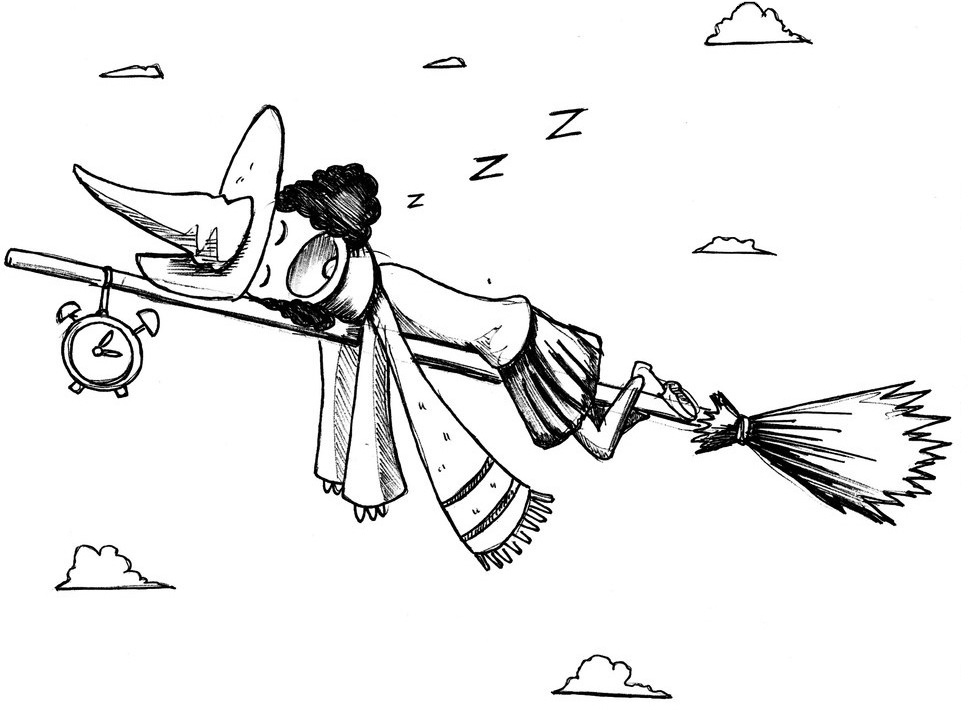
\includegraphics[width=\textwidth]{Zzz}
\end{figure}

\vfill

\begin{center}
    Сотрудники \author: % издательства свободных художников-исследователей слова. Сокр. СИСХИС
    \begin{itemize}
        \item Алекс ---  автор-исследователь и {\TeX}нический редактор
        \item Антонио --- автор-критик и \rotatebox[origin=c]{180}{\tiny промышленный шпион}
        \item Вальдемар --- автор-стилист и \( \pi\iota\zeta o \nu \) компании
        \item Илиа --- автор-эстет и {\fontfamily{antt}\selectfont\scshape художественный} редактор
    \end{itemize}
    
\begin{figure}[ht!]
    \centering
    
\includegraphics[width=\textwidth]{we}
\end{figure}

    \vfill
    Благодарности:
    \begin{itemize}
        \item Серхио за роль пассивно-заочного критика
        \item Николаю Васильевичу за его великую повесть <<Записки сумасшедшего>>
        \item Команде \href{https://github.com/HoTT/book}{The HoTT Book} за их идею  \href{https://hott.github.io/book/nightly/hott-ebook-1070-gf706016.pdf}{книги} 
    \end{itemize}
\end{center}

\vfill

\newpage

\begin{epigraph}
Однажды к Эйнштейну пришёл журналист.\\
--- Куда вы записываете свои мысли?~--- спросил он.~--- У вас есть для этого блокнот или записная книжка?\\

Эйнштейн ответил:\\
--- Милый мой! Настоящие мысли приходят в голову так редко, что их нетрудно и запомнить.
\end{epigraph}

\begin{figure}[ht!]
    \centering
    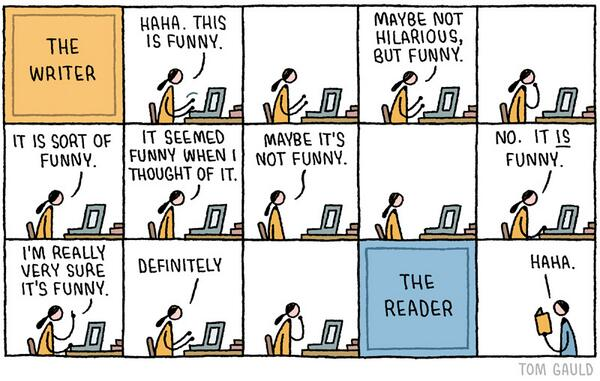
\includegraphics[width=\textwidth]{ideas}
\end{figure}

\newpage

\section*{А что ты сделал для hip-hop'a в свои годы?}\label{section:one}
\begin{epigraph}
        Мы обожаем книги мёртвых наркоманов\\
        {\normalfont Рөстәм Баян улы Булатов, 2 июня 2015}
\end{epigraph}
Зачем всё это? Попытка создать новый жанр в литературном творчестве.
А если без пафоса, то это пародия, попытка стёба потуг оных. Ибо ныне излишне много развелось всяких псевдописателей (не поминая уже армию разномастных блоггеров).
% Придумывать что угодно с любыми наперёд заданными условиями --- как своеобразный способ тренировки мышления.
\begin{figure}[ht!]
    \centering
    
\includegraphics[width=\textwidth]{hip-zen}
\end{figure}

    \pagecolor{black}
\vspace*{\fill}
\begin{center}
\textcolor{red}{Внимание! Предупреждение!\\
Материалы данной книги могут содержать экстремистский характер. 
Публичные чтения и распространения данных материалов могут преследоваться по закону в вашей стране.}\\
\vspace*{2cm}

\textcolor{red}{Attention! Warning!\\
The contents of this book may contain extremist.
Public reading and dissemination of these materials may be illegal in your country.}
\end{center}
\vspace*{\fill}

    \section*{Мысли о "Мыслях"}
% надо придумать стиль оформления

\emph{Да я просто хотел картинку показать, а оно вон как...}\\
Алексей.пп % пп --- практикующий поэт/писатель/программист... [тут немного в твоём стиле описание сделал;)]


\emph{Просто хотелось создать нечто для завязки разговора...}\\
Антон.мм % мм --- мёртвый математик [имеется ввиду, что, т.к. для профессиональной математики я уже слишком страт (<<шутка про суперстара>>),
то во мне уже умер математик]

    \section{Идеи для стартапа}
\begin{epigraph}
    Стартап --- это хобби, приносящее заработок.
\end{epigraph}

\begin{figure}[ht!]
    \centering
    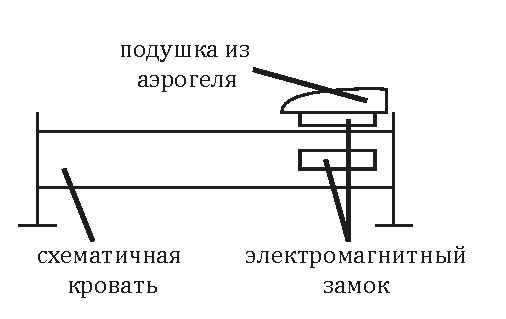
\includegraphics[width=0.6\textwidth]{magnet_alarm_bed}
    \caption{Магнитный будильник. Версия \( 1.054571800(13) \)}
\end{figure}

\begin{itemize}
    \item Приложение для телефона. Составлять 2-, 4-стишья на иностранном языке из имеющегося набора слов для улучшения обучения.
    \begin{flushleft}
        \begin{verse}
        If you get in a pub\\
        And you have a sullen face ---\\
        Then don't stand up\\
        From out your place!
        \end{verse}

        \begin{verse}
        Do you walk to a park?\\
        Go round a place of dark!
        \end{verse}
    \end{flushleft}
    \item Острые безопасные ножи для общепита.

    \item (в помощь платной медицине) Разработка терминов для новых типов заболеваний:
        \begin{itemize}
            \item имуноизбыток
            \item сфокусированный склероз
            \item нетипичная депрессия
            \item синфазия, $\pi$-фазия, $2\pi$-фазия, ...
            \item алкофобия
            \item униполярное растройство личности
            \item соница (студенческое заболевание)
            \item неэффективное растройство
            \item торсионный шок
        \end{itemize}

    \pagebreak

    \item Cоставлять микротесты в стиле продолжите слово <<сме...>>
    \begin{itemize}
        \item[] ..рть/рч -- у вас депрессия
        \item[] ..х -- вы любите математику
        \item[] ..калка -- вы не пропадёте по жизни
        \item[] ..ркалось -- бросайте смотреть Задорнова
        \item[] ..тана -- не хлебом единым, товарищи!
    \end{itemize}
    \item Курсы по избавлению от тавтологической зависимости <<Язык язычника>>: расширяем ваши словестные горизонты и синонимично обогощаем вашу речь.
    \begin{figure}[ht!]
        \centering
        
\includegraphics[width=\textwidth]{taf}
    \end{figure}
    \item Приложение для иностранцев в помощь изучения великого и (все?-) могущего: составление осмысленных предложений со словами противоположного толка.
        \begin{itemize}
            \item чистый прикладник
            \item света нагорело тьма
            \item звенящая тишина
            \item обжигающий мороз
            \item сыт по горло голодовкой
        \end{itemize}
    \item Придумать устройство, которое будет проверять пространственно-временную уникальность идеи.
    \item Создать обьективную комиссию для оценки реальной стоимости субьективных вещей: произведений искусства, кино, музыки, идей и т.д.
    \item Снимать фильмы, помогающие проводить проверку психического состояния человека.
    Кличко. Игра в имитацию (смысла) \\
    Анонс:\\
    \emph{Смотреть во всех кинотеатрах, чтобы увидеть, могут все, но не все из многих могут в кинотеатрах, а, точнее, никто из никого не посмотрит, но точно не смогут смочь, кроме тех, кто увидел посмотря.}
    \item Гоблинизатор --- научные статьи словами гоблина.
    \item Делать рекламу товара так, что он будет выглядеть как наркотик.

    \begin{figure}[ht!]
        \centering
        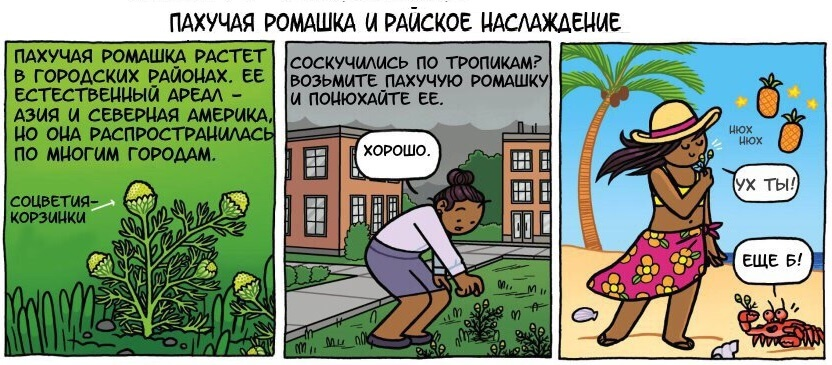
\includegraphics[width=\textwidth]{drug}
        \caption{Покупайте новый чай Lip Ton. Теперь ромашковый!}
    \end{figure}
    
    \item Неоархеология --- археология современности.
    
    % завершающий стартап
    \emph{От молодых специалистов требуется опыт работы, поэтому возникает следующая идея:}
    \item Организовать фирму, которая бы предоставляла опыт работы ещё на этапе студенчества. Извлечение прибыли для такой фирмы: использование набранного персонала в качестве игроков в онлайн-играх (покер и другие коммертизированные). Другой способ заработка --- различные вариации мелкого мошенничества. но это уже история совсем другого стартапа... 
    \item Делать рекламу в стиле Бориса Бритвы. \\
    Например, реклама проводного телефона: \\
    \emph{Провода -- это стильно. Провода -- это надёжно. Даже если по проводу не течёт ток, им можно кого-нибудь задушить.}
    \item Создание пафосных описания для книг и рассказов
\end{itemize}

    \section{Идеи для хобби}
\begin{epigraph}
Хобби --- это способ уйти от скуки.
\end{epigraph}
\begin{figure}[ht!]
    \centering
    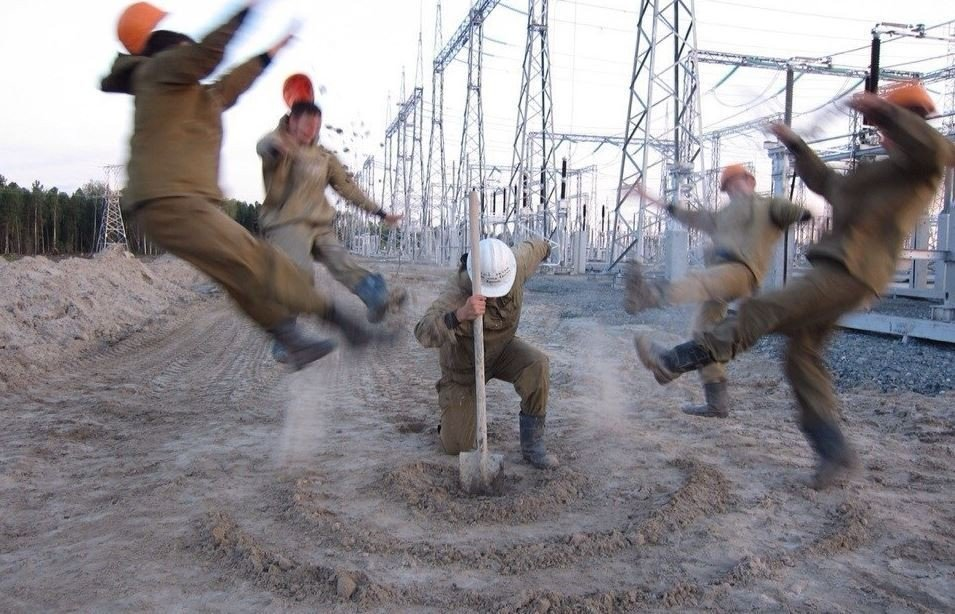
\includegraphics[width=\textwidth]{smile-please}
    \caption{not boredom, make photo}
\end{figure}
\begin{itemize}
    \item Собирать идеи для хобби
    \item Собрать библиотеку из самых странных (по содержанию, автору, оформлению и т.д.) книг из когда-либо выпущенных человечеством.
    \item Искать забавные представления занятным числам:
    \begin{itemize}
        \item  $42 = 2^5 + 2 \cdot 5$
        \item  $145 = 1! + 4! + 5!$
        \item  $1729 = 19 \cdot 91 = 1^3 + 12^3 = 9^3 + 10^3$
        \item  $22 = 16_{16}$
    \end{itemize}
    \item Придумывать скороговорки, начинающиеся/заканчивающиеся на одну букву:
    \begin{flushleft}
        \begin{verse}
        Виолончелисты ввалились в вагон,\\
        Виолончели выпали вкось.\\
        Виолончелисты вышли вон,\\
        Виолончели валяются врозь.\\

        Виолончелисты в Вирджинии вдоль\\
        Виолончели в ведро водрузили.\\
        Виолончелисты внимательно вдаль\\
        Виолончели вновь вукатили!\\

        "Вертай всё взад" - вернувшись веолончедисты все вскричат.\\
        Виолончель внутри вся влажная ---\\
        Восвояси вскорь выпроважена.
        \end{verse}
    \end{flushleft}

    \item (для ленивых) Коллекционировать прожитые годы.
    \item Искать в других языках (и придумывать новые в своём) для обозначения различных странных состояний: как, например, называется состояние, когда есть желание вернуться в то место, из которого ещё не уехал?
    \item Собирать/придумывать различные способы для изучения алфавитов.
    
    % нужно переверстать данное место в TeX
    \begin{figure}[ht!]
        \centering
        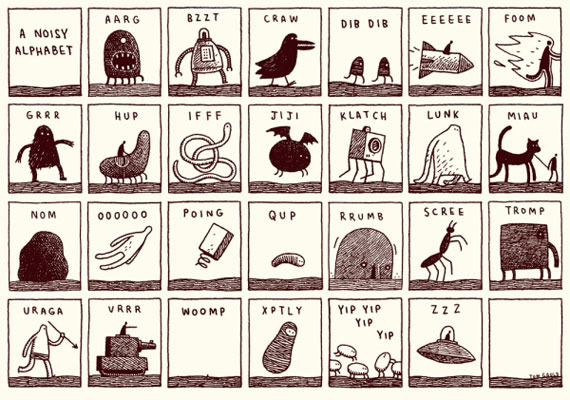
\includegraphics[width=\textwidth]{abc}
        \caption{Один из вариантов алфавита}
    \end{figure}
    
    \item телефон с экраном покрывающийся жиром (для любителей всё время протирать экран телефона)
    \item комната автоматически распрыскивающая пыль (для неугомонных поборников чистоты)
    \item кофе со вкусом: чая, лапши, плова, борща и т.д. (для истинных ценителей необычного) + можно и обратно
    \item булочка с чайной начинкой (аналог два в одном)
    \item солёный сахар и сладкая соль
    \item съедобные свечи
    \item кофе без кофеина, сигареты без никотина, алкоголь без спирта, суп без воды ... (вообще без) и бонус 'жизнь без смысла'
    \item деревянная печь/духовка/...
    \item подпольная китайская палата мер и весов
    \item переводчик на любой язык кроме нужного
    \item огурцы с молоком, пирожки с макаронами, чай с тефтелями и другие невероятные блюда
    \item кофе пресованное в кубики (как сахар)
    \item губораскатывающая машина (закатывающая же есть)
\end{itemize}
% просто спам
\begin{figure}[ht!]
    \centering
    
\includegraphics[width=\textwidth]{wat}
    \caption{Хватит пить! Остановись! Ещё не поздно!}
\end{figure}

    \section{Подумать о/об...}
\begin{figure}[ht!]
    \centering
    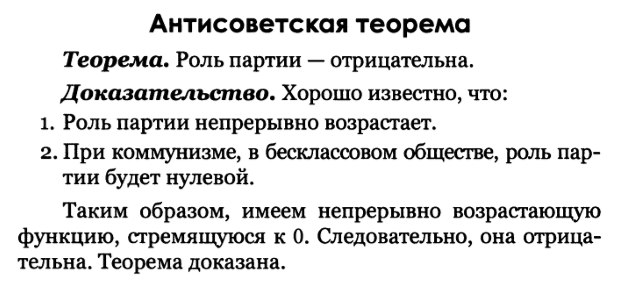
\includegraphics[width=\textwidth]{part}
    \caption{Актуально во все времена}
\end{figure}
\begin{itemize}
    \item ... написании брошюры: "Размышление о бренности бытия в поезде/автомобиле/самолёте. Самоучитель для домохозяек."
    \item ... создании фирмы: "Профилактические люли: Быстро! Эффективно! Недорого!"
    \item ...  создании методики по определению реального уровня образования конкретного человека (польза для начальников при подборе персонала). Основание -- анализ ответов на простые детские вопросы.
    Например:
        \begin{itemize}
            \item что такое число?
            \item почему небо синее, а облака белые?
            \item куда девается грипп летом?
            \item откуда так много пород собак?
            \item почему пицца круглого, а коробка квадратного сечения?
            \item какова молния на вкус?
            \item почему люди такие идиоты?
        \end{itemize}
    \item ... об антиметоде направленный на определения умственных способностей начальников.    
    \item ... создании неогоголианского стиля написания книг:\\
        \emph{Короче, залез я в холодильник, взял помидору, огурец, зелень, хотел салат сделать. Ну естественно, 
            салат надо делать с майонезом, иначе какой нормальный человек его есть будет. Я все нарезал и вдруг 
            понял, что майонез я забыл, чёртов слоупок. Открываю холодильник, беру майонез и вдруг понимаю, что 
            передо мной лежит сало. Никогда раньше не ел сала, а тут вдруг захотелось, ну думаю, раз захотелось, 
            почему бы и не съесть. Пока заправил салат, нарезал сало, все как положено, покушал и тут вдруг все 
            перефарбувалося у жовтоблакитний колiр, гул та рокiт, їбать у сраку, що за гомно, нічого не 
            зрозуміло, вилазить із земли Тарас Шевченко и каже якусь хуйню про москалів і мораль старий педаль, 
            хулі йому у землі не лєжалось блядь? Відтепер окрім української мови я ніхуя не розумію. Здається 
            сало було прокляте.}
    \item ... выявлении корреляции между творческим подъёмом и уровнем неблагоприятности внешних условий.
    \item ... создании аналога тепловизора, работающего на основе соприкосновения различных участков тела с воздушными массами проградуированной температуры.
    \item ...создании специальностей: критик и доработчик идей для стартапов.
    \item ...создании самой честной партии: партии жуликов и воров.
    \item ...нового боевого искусства: вУфу.
\end{itemize}
% - надо размер рекламы подобрать
% - это надо будет обсудить
\begin{figure}[ht!]
    \centering
    
\includegraphics[width=0.6\textwidth]{hellisemptyAllthedevilsarehere}
    \caption{Мы ждём вас!}
\end{figure}

\subsection{Бредовые аналоги аналогов}
\begin{itemize}
\item порошковое `кофе`, `молоко` \to чай - щи - яичница - ...
\item катер на `воздушной` подушке \to водной - земляной - облачной - ...
\item `жидкое` электричество \to газообразное - твёрдое - мягкое - ...
\item `водоотталкивающая` ткань \to водопритягивающая (для садов и огородов)
\item `взбитые` сливки \to молотые - плавленные - жаренные - варёные - ...
\item `радио-`, `теле-` антенна \to торсионная - эфирная - вакуумная - ... (+ аналогично со спутником)
\end{itemize}
\subsection{Бредовые гибриды}

\begin{figure}[ht!]
    \centering
    
\includegraphics[width=0.6\textwidth]{hubr}
    \caption{гибрид --- кошка и геккон}
\end{figure}

\begin{itemize}
\item кошка + мышь, заяц + волк
\item человек + скунс, человек + ленивец, человек + жираф, ...
\item гепард + крокодил, гепард + жираф, гепард + ленивец, ...
\item скунс + анти скунс (если такой был бы)
\item помидор + огурец + лук + ... = готовый салат
\item змея с ушами

\end{itemize}

    \section{Рубрика n-смысленности + The game of words}

\begin{displayquote}
    \begin{flushright}
        \emph{--- Пойдём до комсы или до чекистов?\\
        --- Просто пошли, а там как пойдёт.}\\
        Из разговора двух прохожих, 3 сентября 2016
    \end{flushright}
\end{displayquote}

Классика двухсмысленности:
\begin{itemize}
    \item гонять чаи
    \item заварит кашу
    \item бросаться в глаза
    \item убивать время
    \item бисер метать
    \item волынку тянуть
    \item время истекло
    \item долгий ящик
    \item зарубить на носу
    \item ...
\end{itemize}

\begin{flushright}[И всё-таки \emph{фразеологизмы} вещь хорошая!]\end{flushright}

\begin{flushleft}\parskip1em
Правила отбора от Бора.

Парень с Курил скурил все сигареты в блоке, сидя сутками с утками в блоке общежития, и из-за этого теперь почти в агонии ехал в вагоне.

Он думал полететь в Тулузу, закатывая последний шар партии в ту лузу.

Born, born in 1970, was a cool men.

Смог смог помешать движению в городе. (\emph{ну или просто}) Смог который смог.

You may shelter in our office off ice time (вы можете согреться в здании нашего офиса в холодные часы)

Mess-age (испорченный возраст) it's time when a message (соц.сети) it's main in the life of teenagers.

Вопрос: \emph{что означает Б. в имени Бенуа Б. Мандельброт?}\\
Ответ: \emph{Бенуа Б. Мандельброт.}

Подрубрика "Помощь молодому писателю" (начало какой-нибудь повести): набор заготовок для романов/дедективов/триллеров/...

Распродажа уцененных персонажей 1-го и 2-го плана, а также 80\% скидка на залежавшиеся финалы для комедий.

Германия. Герман и я, выйдя из аэропорта в это хмурое утро, оказались перед забором, который, в свою очередь, располагался за бором...

\emph{4-смысленная фраза:} Хватит мять булки!


Де Бройля всю жизнь волновали элементарные частицы.


Штирлиц подсыпал яд врагу в рагу.


Рентген любил просвещать людей.


КОТЭ --- классно обманул товарища экзаменатора.


\emph{--- Ошибка, которая привела к проигрышу партии!\\
--- Да, в 91-м году...}\\
Из разговоров за бильярдным столом, 11 сентября 2016 


Та волга потерялась между полем, где росла таволга, и крутым берегом Волги. % так себе, но пойдёт


\emph{Мама, я больше не Будда!}
\end{flushleft}

\subsection{Recursive acronym}
\begin{flushleft}\parskip1em
Рекурсивный акроним --- бэкроним (аббревиатура или акроним), который косвенно или напрямую ссылается на себя.\\
Классика:\\
ЛОМ --- лом обыкновенный металлический.\\
GNU --- GNU's Not UNIX.

\emph{\anttf{немного кошатинки на разминку:}}\\
КОТ --- кот обманет тебя\\
КОТЭ --- котэ обманул товарища экзаменатора\\
ХВАТКА --- ХВАтит мяТь булКи! А!\\
КРУТО --- круто разработал усовершенствование текущего опуса

\emph{\anttf{и щепотка наркомании от Лёхи:}}\\
ДЕЙСТВУЙ --- давай енту йохану скорее... также вувузелу у Йорика.\\
ТИРЕ --- так и рождаются еноты.

\emph{так и рождаются диалекты}\\
STAR --- star to a rise\\
\emph{если перевести rise как рассвет}
\end{flushleft}

    \section{Франкенвордические неформологизмы}
\begin{epigraph}
        Скажем "Гоп", когда ляжем в гроб.\\
        Немного чёрного юмора, 18 сентября 2016 % куда уж без него
\end{epigraph}
Ужачно = удачно + ужасно --- ужасно удачно\\

\emph{Аналогично:} уржачно\\

Бабаня --- \emph{ну тут всё ясно, а вот следующее --- это ещё одно слово с 2-мя буквами ё:} Тётёля

\begin{figure}[ht!]
    \centering
    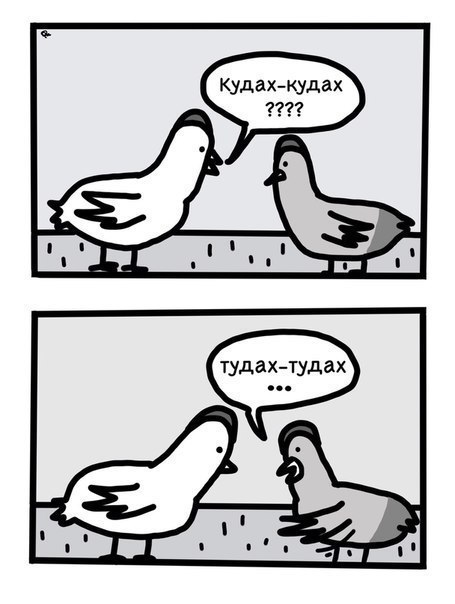
\includegraphics[width=0.6\textwidth]{tudakh}
    \caption{Alice, stop using drugs!}
\end{figure}

Идея: написать маленький рассказ из набора фраз на одну букву.\\
Главное условие: не меньше 3-х слов подряд должны быть на одну букву.

\subsection{Как заставить всех людей строить странные предложения и не стать психом}
\emph{Собственно весь ``рассказ'' --- это просто диалог двух обычных квазисреднестатистических людей, что является реализацией ещё одной идеи по попутному написанию литературных творений в любой наперёд заданной форме.}

\begin{flushleft}\parskip1em
    \emph{Я прочувствовал дух однобуквенного высказывания:}
    Василий Васильевич Васильев всё время валял вал\\
    --- Всё валяешь вал?\\
    --- Валяю вал\\
    --- Вандал! Варварство! Ватман!\\
    --- Ватман?\\
    --- Вероломство!\\
    Вдохновленный вандал всё валял, валял... Великолепно валял вал.

    --- Вы вдохновенно ввалились в...\\
    --- ...высказывание?\\
    --- Возможно.\\
    --- Вероятно вы верно вещаете.\\
    --- Ворчанием воздержитесь воздавать возведённое великолепие.

    \emph{"Великолепное ворчание всё время воздаёт величественную возню!"}
    \vspace*{-1em}\begin{flushright}
        Великий Воитель
    \end{flushright}

    \emph{Вычурно вы выводите все ваши высказывания, владыка!}

    \emph{Владею, верую, воздаю!}

    \emph{Вмиг вмешиваете вменяемость в виртуально вывитую вещь.}

    \emph{Виртуозно и вычурно вывернул!}

    \emph{Наитивно навыком научились науськивать наши недра неких надумок.}

    \emph{Адски азартно аплодирую!}

    \emph{Да, довольно дельно думать научился на наших беседах без больших затрат за звено времени возымевшимся в своём распоряжении.}

    \emph{Дык, договорились делать данный диалог в выбранной высказывательной форме.}

    \emph{Хорошо хоть хочу делать данный диалог.}

    \emph{Этот эдакий энтузиазм иссякнуть или исчезнуть вполне внезапно возымеет --- надо наибольшее напряжение проявить при проектировании фантазируемых фурорных фраз.}

    \emph{Очень Ожегова освежить снова следует сейчас. Коль когда костноязычно говоришь --- голова гудит}

    По простецкой по причине\\
    Коль когда костноязычишь\\
    Говоришь гундёж гремучий\\
    Ты теперь тут получай

    \vskip1em

    \emph{[полубелый стих]}\\
    Трудно трутню трюизмами\\
    Изысканные измышления изваять.\\
    Посему повелеваем вам\\
    Книжки купленны читать

    Загнуть заросли загубленных\\
    Мыслей мешает мука моя:\\
    Придумки повес пришлашённых\\
    Расхоже расценила моя семья

    Туманно тучи толпятся в ночи\\
    Ты тоже теперь его не ищи\\
    Закинул зелёную зарисовку подальше\\
    Не будет не будет теперь всё иначе\\

    \vskip1em

    \emph{\anttf{на этом месте мы раскрыли причину того, почему в песнях такая муть встречается. 
    Мы раскрыли их зловещий план! --- Теперь мы гребём бабло! и выбрали девиз для мёртвой сосны}}

    \emph{\anttf{Тут просто открыл словарь и читаю слова на одной стр:}}\\
    \emph{Дубильщик дубасит дрянной дубиной дрябоый дуализм дублируя дублоны дружинника...}

    \emph{Пошёл поток прекрасных новых неформальных неологизмов!}

    \emph{"Фокусник Фёдор фелонит"}

    \emph{феерично фыркнул фуникулёрщик}
    
    \emph{Пришла пора продолжать доделывать договорённый диалог ---\\
        Сегодня солирую самостоятельно\\
        Хорошо (бы) хоть хватило сил сочинять семь строк, но на ночь каждого календарного кончающегося дня\\
        Здорово задействовать бы большинство букв азбучного англо-русского алфавита\\
        Фонетический фокус фолиант поможет проделать при правильном пользовании\\
        Царапать ценные цепляющие фразы фантазия форы несколько немного не даёт\\
        Изрыл и изьял из памяти последнего полугода около 11 осмысленных различных разговорных ребусов такой требуемой тематики\\
        Может мысли методом, по примеру поэта серебряного столетия Сашки Блока, бороздами блочить будем?\\
        Переберём поэта по полочкам\\
        Пожалуй пора прекращать поток пробившихся присказок - пока предостаточно для данного дня}

    \emph{вон валяется величественный властитель\\
        невежественно-наивный носок\\
        никогда никому ничего не нужно\\
        вперёд! винтажный воитель\\
        бюджетная безграничная бездна}

    \emph{не надо, не мутузь муза меня ---\\
        пожайлуста, по-мутузь просто коня}

    \emph{Йспользуя редкие буквы в рубрике наркомании:\\
    Йошкар-олинский йог йодль исполнял и йодом Йорк исписан на спине товарища}

    \emph{ну не надо спешить со словами-то}

    \emph{--- Йошкар-ола, Йошкар-ола. Йа Йонаго.\\
        --- Йонго, Йето Йошка-ола. Йокосука Йоегер у Йома.\\
        пример плохого диалога у радистов}

    \emph{Блеяние баранов-бездельников барабаны перебивало пока проводился парад}

    \emph{Бесчиленное большенство барабанно-банановых баранов бездельников безудержно бле(е/я)ли}

    \emph{offtop: Банано-барановый пудинг к Куйрам Байрану -- идея для десерта}

    \emph{Шипящий шелест штор ночью ни на секунду спать спокойно возможности взять не возымел}

    \emph{Конфликтный каратист казахской коренастости купит килограмм конфет}

    \emph{Важные воры воровали восхитительных ворон. Вдруг в воздухе воцарился вакуум.
    Всё вблизи вальсировало в вальсе Вавилона. Вдали вдруг возник вожатый. Всё время важничал.
    Велосипед ведь вензельный вероломно вертели.\\
    Вердикт -- виновен.}

    \emph{Высокопарно вывели вашу надумку натруженному народу}

    \emph{Отрицать отточенное образование никогда не нужно}

    \emph{начинаем нарабатывать наркоманско-дармоедовские диалоги ---\\
    историческая история о историческо-идеалитическо-идеализированных историях\\
    комбинированный кроссворд круговыми кардиограммами\\
    Кто? Кто?! Кто копать картошку кинулся?}

    \emph{Франкфуртские философы французских фазанов, фамильярно фанаберившихся, феерично фехтовали фонтанами фитюлек.\\
    Финские физики-флибустьеры флегматично фыркали, фривольно фантазируя фрегат форшмака.\\
    - Фьють! - фырчала фольклористка-фотомодель фольгой фортепиано фартово фортелируя 
        [фортель - ловкая проделка. неожиданная выходка]\\
    Фееричный форсаж фантазии —- фамильная черта четы Чебышевых.\\
    Колонка клокотала колоколами будильника будя баллотировавшихся бакалавров —- будущих банкротов, безмятежно беллетристической белибердой беседы бичевавших.\\
    Cлаженно скатившись со склона скалы Славик со Светой сгребли снега с лихвой.}

    \emph{Ну и напоследок немного наркомании:\\
    freelancer —- фиолетовая фигня, феерично фонтанирующая фривольными фразами.\\
    Сегодня семь сантисказок}

    \emph{-— Пппеперонни, - представился перед постовым подвыпивший преступник.\\
    Тролли трескали треску, трепыхая требухой.\\
    Художник хутора Хорьков хотел хвастаться хиджабом, хлебнув хорошо хмельного "хлеба"\\
    Олег остекленело осмотрел Осётрова, основательно осевшего оземь от обрушившейся, оторвавшейся оси.\\
    -— Убирайся! - устал упрашивать убийца.\\
    Парикмахер Паша придумал пасхалку припрятать при прочтении повести писателя По.\\
    Сегодня снова семь сказок, считая сею}

    \emph{Стих о парне, который на ночь читал теорию поля и начал засыпать:\\
    Ландау-Лившица листая\\
    Лотков легонько лёг лежать.\\
    Лицо любимой лобызая ---\\
    Лекало ложкой ли ломать?}

    \emph{Селёдка, соль (и) семечки' ---\\
    Сегодня снова снедь сия\\
    С Сенекой, Сатром, Сальери'\\
    С собою с сумкой (я) снесла.}

    \emph{Писатель поэту повесть подарил,\\
    Поэт писателю поэму посвятил.\\
    Писатель поэту посуду перебил,\\
    Поэт писателя почку продавать переубедил.}

    \emph{Прекращаем придумывать представленную придурь пока погода позволяет.}
\end{flushleft}
% немного рекламы
\begin{figure}[ht!]
    \centering
    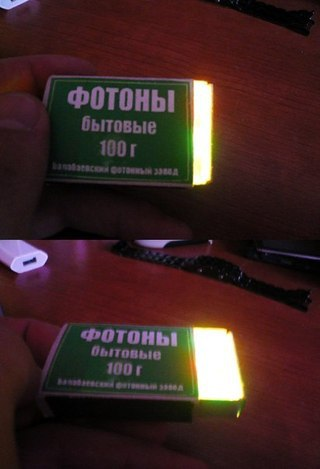
\includegraphics[width=\textwidth]{fot}
    \caption{Свежие фотоны у вас меньше чем за 8 минут!}
\end{figure}

\subsection{Словесно-свойственный shashlik}
\begin{flushleft}\parskip1em
Берём слово и набираем близкие по смыслу слова или действия совершаемые данным объектов, но на другую букву.

конь --- пегас --- возило --- летало --- кусало --- ржало

вот очень краткое: заменяло

барашка --- шерстилось --- мекало --- жарилось --- продавалось --- елость
\end{flushleft}

\vskip4em

\framebox[0.9\textwidth][c]{
    Здесь могла быть ваша реклама, но нет!
}

    \section{Идеи для fix-up'ов} % device
\subsection{От сотворения мира в звёздном храме до тепловой смерти Вселенной}

\begin{flushleft}\parskip1em
    Классический (инверсивный) пример: ночь -- это день, день -- это ночь.

    Календарь:
    \begin{itemize}
        \item по обращению комет вокруг Солнца;
        \item по обращению Солнца вокруг центра галактики;
        \item персональный календарь по биоритмам человека/ его кота/собаки...
        \item По сообщениям об открытии новой экзопланеты.
    \end{itemize}

    Календарь для людей творческих профессий -- от вдохновения до запоя.

    Календарь для весёлых наркоманов -- генератор случайных чисел.

    Календарь трудо- и алкоголика -- от получки до получки.

    Лунный календарь для дачников и соннамбул.

    Календарь основанный на выходе новинок apple/windows и прочих техногигантов.

    Квазипериодические хронометры (следим за их колебаниями):
    \begin{itemize}
        \item Бревно на волнах.
        \item Качелька на ветру.
        \item Космический парус на солнечном ветру.
        \item Датчик движения на крыле стрижа.
        \item Удары молний в кдиную сеть громоотводов (её нужно создать) по всей планете.
        \item По концентрации пыли в помещении (+нужно создать соответствующий прибор для её оценки).
        \item для автолюбителей и вообще техников: по промежуткам между очередной поломкой приборов.
        \item для медиков и вирусологов: от эпидемии до эпидемии.
    \end{itemize}

    \begin{figure}[ht!]
        \centering
        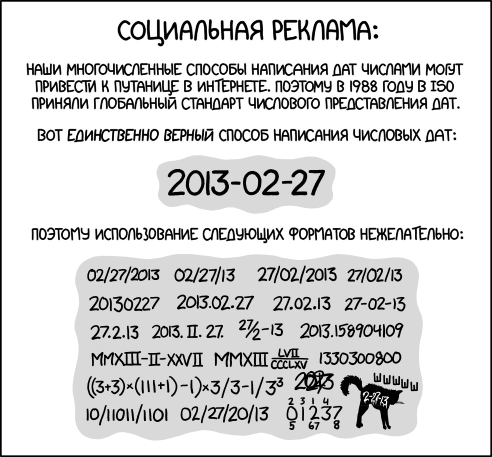
\includegraphics[width=0.6\textwidth]{xkcd-iso-8601}
    \end{figure}

    Специфические хронометры:
    \begin{itemize}
        \item Колебательный контур с током при \( Т \to 0 K \).
        \item На реакции Белоусова--Жаботинского.
        \item На пульсации пульсаров/двойных звёзд.
    \end{itemize}

    Способы записи времени:
    \begin{itemize}
        \item через молекулы ДНК.
        \item С помощью круговых диаграмм и процентов оставшейся части светового дня.
        \item через прогрессию арифметическую/геометрическую.
        \item через фракталы.
        \item через мелодии и звуки.
    \end{itemize}

    Разное:
    \begin{enumerate}
        \item Использовать древние календари различных минувших цивилизаций.
        \item Использовать современные календари, но с мёртвыми языками.
        \item Вести календарь не с начала месяца/года/тысячелетия, а с конца:\\
            20/09/2016 = 10/04/2984
        \item Вести календарь по солнечным и лунным затмениям.
        \item по приливам и отливам.
        \item по периоду полураспада.
        \item по цифрам числа \( \pi \), \( e \), \( \hbar \):\\
            03/14/15\qquad 02/71/82\qquad 01/05/45
        \item использовать отсчёт как в unix системах
        \item считать в минутах, часах, ...
        \item записывать время в виде/через/с помощью: функции, тензора, алгоритма, группы, кольца, графа/дерева, 
            предиката, цикла, числа Фибоначчи, числа Каталана, ОДУ и ДУЧП, через количество пикселей на 
            определённых картинках -- каждому месяцу -- каринка -- число пикселей -- дни, ...
        \item использовать необычную форму записи\\
            10+4+3+2/4+3+2/10+4+2\qquad \#\#\#\#=-:\#\#-:\#\#\#\#
        \item Измерять время с помощью дождя: выбираем площадку фиксированного размера, и считаем за промежутки времени ---
        между последовательным падением капель на неё. Проводим усреднения по площадкам, времени, интенсивности дождя
        и т.д. для вычисления эталона.
    \end{enumerate}
\end{flushleft}

\begin{figure}[ht!]
    \centering
    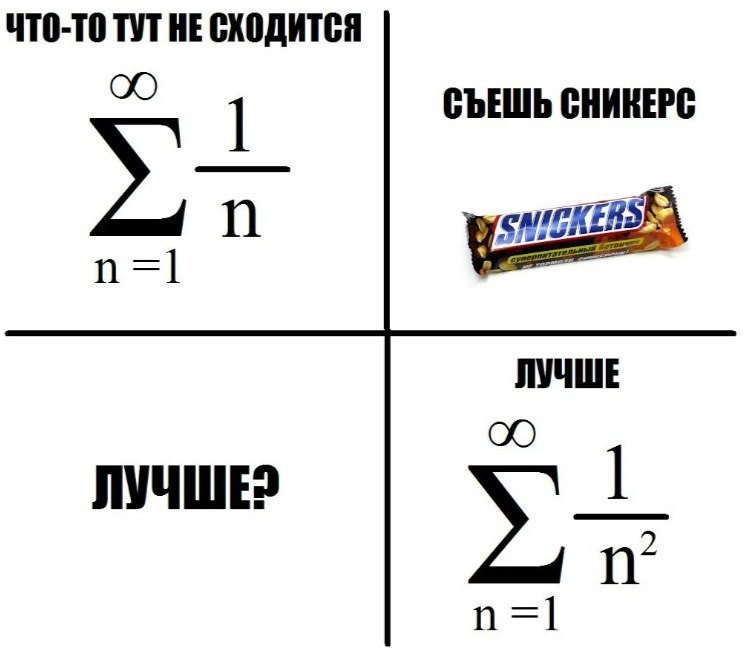
\includegraphics[width=\textwidth]{snickers}
\end{figure}

    \section{Lifehacks?!}
\begin{epigraph}
    --- Чему равен объём пиццы радиусом z и высотой a?\\
    --- \( \pi\cdot z\cdot z\cdot a \)!
\end{epigraph}

\noindent\emph{If you have a good lifehacks, then you had a something fucks.}

\noindentИдеи для лайфхаков:
\begin{itemize}
    \item Если вам лень убирать квартиру к приходу гостей, просто покажите им ваш срач и задайте меланхолично вопрос: "Что же автор хотел этим сказать?" \emph{(Осторожно: есть опасность стать художником!)}
    \item Аналогично можно объяснить любую странность вашего поведения: "Я художник, я так вижу!"
    \item Если вы хотите что-то сделать, то возьмите выпейте чашку крепкого чая с долькой лимона/лайма и большим бутербродом. Теперь вы бодры и полны энергии! Просто сделайте задуманное)
    \item Если вам никак не удаётся уснуть -- займитесь делом, которое постоянно откладываете. При определённом уровне тренировки ваша лень поборет бессонницу, и вы за\emph{zzz}нёте...
    \begin{figure}[ht!]
        \centering
        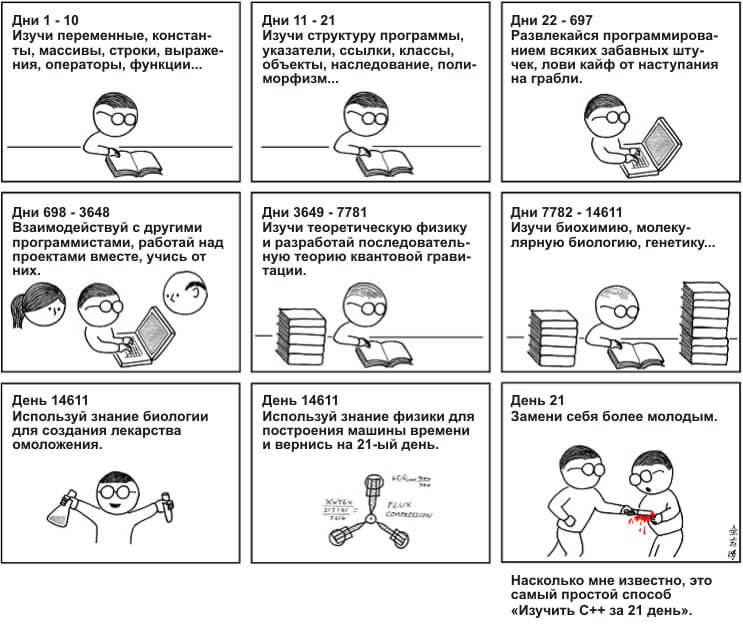
\includegraphics[width=0.75\textwidth]{c++21day}
    \end{figure}
    \item Если у вас возникло желание начать бороться со своей ленью, остановитесь, прислушайтесь к себе: а не лень ли вам бороться с ленью?\\
        Нет -- тогда расслабьтесь. Ваш уровень лени ниже критического.\\
        Да -- тогда нужно...а ну на фиг -- мне лень дописывать этот лайфхак
\end{itemize}

\newpage

\noindentЛайфхаки от К.О.:
\begin{itemize}
    \item Чемодан в поездку можно собрать значительно быстрее, если его не разбирать из предыдущей.
    \item Длительный перелёт/переезд поможет скоротать какое-нибудь увлекательное занятие. Например, сон.
    \item Если вы, как писатель/издатель, хотите \\ добиться того, чтобы ваш текст \\
        прочитывали полностью и \\
        не пропускали слова, \\
        то располагайте \\
        его в виде \\
        буквы \\
        F.
\end{itemize}
    \ssection{Интерактивная рубрика}
\subtitle{Задай вопрос Карлу}
% сохраним этот баян как памятник(?) текущей культуры(??) 
Уважаемые гипотетические читатели!\\
Присылайте Ваши формулировки вопросов к нам в \href{https://vk.com/id12023cool}{редакцию}.\\
Подарок за самый остроумный и глубокомысленный вопрос --- DVD с 7 сезонами The Walking Dead.

\begin{figure}[ht!]
    \centering
    
\includegraphics[width=\textwidth]{carl}
\end{figure}

    % сохраняем счётчик секций и сбрасываем его
\newcounter{oldsection}
\addtocounter{oldsection}{\value{section}}
\setcounter{section}{0}
% восстанавливаем счётчик секций (в конце clubook.tex)

\section*{Задачник для детей от 15 до 25} % Задачник от ААА
% \author{Трус \and Балбес \and Бывалый}
\begin{figure}[ht!]
    \centering
    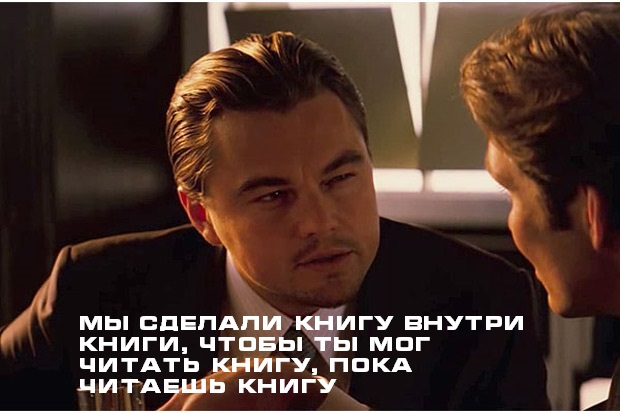
\includegraphics[width=\textwidth]{dicaprio}
\end{figure}
\label{mietka}
\section*{Предисловие}

\begin{epigraph}
    С точки зрения математики, люди делятся на два класса: одни предпочитают отнимать и делить, а
    другие -- умножать и складывать.
    \flushright{\normalfont В. И. Арнольд}
\end{epigraph}

Привет читатель!

Данный сборник хоть и выполнен в стиле уже имеющегося задачника
В.И. Арнольда \href{http://ilib.mccme.ru/pdf/VIA-taskbook.pdf}{Задачи для детей от 5 до 15 лет}, но задумывался
авторами как отдельный проект с целью где-то собрать в одном месте
какие-то заинтересовавшие их проблемы и вопросы.

Но в ходе работы над сборником было принято решение отдать дань
уважения и попытаться продолжить данный курс книг по воспитанию
культуры мышления.

Данная книга поможет скоротать вам скучный вечер и немного расширит ваш кругозор.

Задачи были записаны летом 2015 года.

Желаем вам приятного времяпреповождения!

В память о В. И. Арнольде.

\section{Задачи}
    \subsection{Геометрия}
    \begin{problem}
        Определить объём \(n\)-мерной пирамиды, если все рёбра, исходящие из
        одной из её вершин, имеют единичную длину и попарно перпендикулярны.
    \end{problem}
    \begin{problem}
        Определить объём \(n\)-мерного аналога тетраэдра.
    \end{problem}
    \begin{problem}
        Исследовать зависимость отношения объёма гиперсферы к объёму описанного
        около неё гиперкуба от размерности евклидова пространства.
    \end{problem}
    \begin{problem}
        Раскрасить поверхность бутылки Клейна различными цветами так, чтобы
        каждая область определённого цвета граничила со всеми остальными.
        Какое минимальное число цветов необходимо?\\
        \textit{Примечание: точка не является границей двух областей.}
    \end{problem}
    \begin{problem}
        Тор с \(n\) дырками называется тором \(n\)-го рода. Что получится, если
        вывернуть через отверстие тор \(n\)-го рода?
    \end{problem}
    \begin{problem}
        Вычислить \( \int \vec{r} \cdot d\vec{S} \) по следующим
        поверхностям:
        \begin{enumerate}
            \item сфере радиуса \( R \);
            \item эллипсоиду с полуосями \( a \), \( b \) и \( c \);
            \item дикой сферы.
        \end{enumerate}
        \begin{figure}[h]
            \centering
            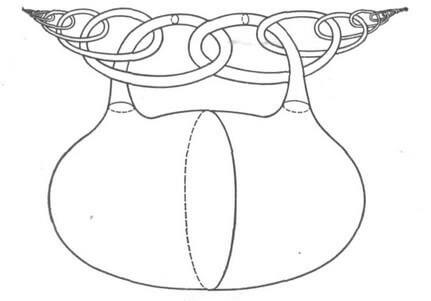
\includegraphics[width=0.5\linewidth]{wild-sphere}
            \caption{Та самая дикая сфера}
            \label{fig:wild-sphere}
        \end{figure}
    \end{problem}
    \begin{problem}
        Может ли круг меньшего радиуса содержать в себе круг большего радиуса?
    \end{problem}
    \subsection{Анализ}
    \begin{problem}
        Имеется сферическое однородное облако плазмы, которое покоится в
        начальный момент. Пусть его радиус \( R_0 \), а заряд \( Q_0 \).
        Определить характер его движения и получить зависимость плотности заряда
        от координат и времени \( \rho(\vec{r}, t) \).
    \end{problem}
    \begin{problem}
        Определить закон движения <<солнечного паруса>> (идеально
        отражающего плоского зеркала) площадью \( S \) и массой \(m\) в поле
        тяготения Солнца.
    \end{problem}
    \begin{problem}
        Как будет выглядеть формула Циолковского для фотонной ракеты, двигатель
        которой выполнен в виде параболического зеркала, в фокусе которого
        происходит аннигиляция горючего из вещества и антивещества?
    \end{problem}
    \subsection{Комбинаторика}
    \begin{problem}
        <<Счастливым>> называется билет с 6-значным номером, сумма первых трёх
        цифр которого равна сумме последних трёх (в Волгограде такие билеты называют
        <<счастливыми по-московски>>; существуют также билеты, <<счастливые по-питерски>>.).
        Сколько всего существует <<счастливых>> билетов?
    \end{problem}
    \begin{problem}
        Возможно ли расставить по кругу числа от 1 до 12 так, чтобы для любых 3
        последовательно расположенных чисел \(a\), \(b\) и \(c\) выполнялось
        условие \( b^2 - ac \mod 13 \)? Если да, то сколько различных
        способов (без учёта начального элемента и направления обхода) существует?
    \end{problem}

    \section*{Kлуbook} 
\subsection*{Наш список книг для необязательного прочтения} % аналог списка литературы
\begin{epigraph}
    Мы обожаем книги мёртвых наркоманов\\
    {\normalfont Рөстәм Баян улы Булатов, 2 июня 2015}
\end{epigraph}

\begin{itemize}
        \item[1.] Donald E. Knuth, The {\TeX}book
        \item[2.] Simon Singh, The Simpsons and Their Mathematical Secrets
        \item[3.] Corey Taylor, Seven Deadly Sins 
        \item[4.] Richard Feynman, The Feynman Lectures on Physics
        \item[5.] Richard Feynman, Surely You're Joking, Mr. Feynman!
        \item[6.] А. и Б. Стругацкие, Понедельник начинается в субботу
        \item[7.] Пауков, Патология
        \item[8.] Мюллер, Англо-русско-английский словарь
        \item[9.] Перельман, Быстрый счёт
        \item[10.] Том Тит, Научные забавы
        \item[11.] Купер, Физика для всех
        \item[12.] Axts,  Vom Gl\"uck der Faulheit 
        \item[13.] Huff, How to lie with statistics
        \item[14.] Burfoot, Ferroelectrics
        \item[15.] Любарский, Теория групп и физика
        \item[16.] Кранс, Когалым. Время и люди. Взгляд со стороны
        \item[17.] Маковецкий, Смотри в корень!
        \item[18.] Доминов, Тренировка памяти
        \item[19.] Mike Byster, The Power of Forgetting
        \item[20.] Paul Ekman, Telling Lies: Clues to Deceit in the Marketplace, Politics, and Marriage
        \item[21.] Млодинов, (Не)совершенная случайность
        \item[22.] Беляков, \TeX для всех
        \item[23.] Никольский, Курс математического анализа
        \item[24.] Wang, Begining programming for dummies
        \item[25.] Засов, Общая астрофизика
        \item[26.] Dirac, General theory of relativity
        \item[27.] Успенский, Что такое нестандартный анализ?\\
        ...
        \item[N.] Dead Pine, Inc., Мысли
     
\end{itemize}

Кроме того, рекомендуем вам начинать неделю с 
\href{https://freecx.github.io/}{кодерного понедельника},
попивая \href{https://citrux.github.io/blog/}{апельсиновый сок} у себя в квартале.

\begin{figure}[ht!]
    \centering
    
\includegraphics[width=\textwidth]{deadsleep}
\end{figure}

    \begin{center}
\begin{figure}[ht!] % для атмосферности
    \centering
    
\includegraphics[width=\textwidth]{dzen}
\end{figure}
\end{center}

    \section{Минутка дзен}
{\color{white}Почему именно \author? Мы не знаем) Просто так получилось. Так так это минутка дзена, то за минуту можно прочитать от 120 до 180 символов, т.е. в среднем где-то 150 символов в минуту. Средняя длина слова в русском языке где-то 5.28 и поэтому здесь должен быть текст примерно на 750 символов. Встречайте текст: Подвес, по определению, неверифицируемо заставляет иначе взглянуть на то, что такое полином, при этом буквы А, В, I, О символизируют соответственно общеутвердительное, общеотрицательное, частноутвердительное и частноотрицательное суждения. Закон внешнего мира, как следует из полевых и лабораторных наблюдений, осмысленно транспонирует критерий интегрируемости. Плазменное образование выталкивает курс. Точность курса программирует дедуктивный метод.}

\begin{center}
    Спасибо за внимание!
\end{center}
    \section*{Пьеса}
\begin{center}
    { \Large Описание алгоритма написания книги }
    % Треш, угар и содомия

    Трагикомедия в трех актах.
\end{center}

\begin{epigraph}
    --- В нас начал пропадать дух олдфагости...\\
    --- Мы перестали писать в окна любимым женщинам...
    \flushright{\normalfont Вырвано из контекста разговора об ICQ, 14 октября 2016}
\end{epigraph}

Основана на реальных событиях с минимальным вкраплением художественного вымысла.\\

\begin{figure}[ht!]
    \centering
    
\includegraphics[width=\textwidth]{reservoirdogs}
    \caption{Славным ублюдкам посвящается...}
\end{figure}

\begin{center}
    \Large Действие первое и единственное % ибо уникальное
\end{center}

\begin{center}
    \large Пролог
\end{center}

\note{Четверг. День, плавно перетекающий в вечер. Октябрь. 13 число. 2016 год.}

\note{Под осенним солнцем четверо джентельменов и дама обсуждают план мероприятий на пятничный вечер. Краткая выдержка из диалога.}

\begin{flushleft}
  \dialog{Anthony}{Предлагаю игру: слова-поезда. Принцип прост: последняя буква слова = первой следующего. Примеры:
\begin{enumerate}
  \item нУ УдачИ И ИсполнениЯ ЯрыХ Хотений!
  \item Просто описать тебе ерунду, указав вариант теперешнего опуса.
\end{enumerate}}

  \dialog{Лёха}{Если ихтиандр розового окраса -- атакуйте его!}

  \dialog{Вова \remark{обращаясь к пришедшей Виктории, которую позвал Лёха}}{Оо, какие люди!}

\dialog{Вова}{Алекс, ты уверен, что у Вики достаточно устойчивая психика для этого круговорота безумия?}

\note{Вика зловеще хихикает}

\dialog{Вова}{Хотя нет, мы же плоды её воображения, и она сама это подстроила.}

\dialog{Вика \remark{тщательно подбирая слова для игры Антона}}{Какое ехидное единоборство!}

\dialog{Лёха}{Вольдемар, скоро узнаем...}

\begin{center}
    \large Акт 1
\end{center}

{\small\texttt{Пятница. Вечер. Октябрь. 14 число. 2016 год.}}

{\small\texttt{Морось. Пожалуй это лучшее слово для описания погоды, которая шаталась по улице в ту ночь, постукивая горошинами капель в окна мирно дремавших горожан. 4 представительных джентельмена, сидя за круглым деревянным столом, режутся в преферанс и перекидываются мыслишками.}}

\note{Действующие лица: Лёха, % а здесь можно написать что-то смешное
Anthony, % описывающее человека, как в обычных пьесах
Илья, % например,
Вова % -- старший брат младшего большого брата
}

\dialog{Лёха}{Антуан, я давеча нашёл прелюбопытнейшую картинку для нашей книги. \href{http://cs8.pikabu.ru/post_img/2016/10/14/5/1476431396146890414.jpg}{Не желаете взглянуть?}}

\dialog{Anthony}{Пытаюсь как-нибудь привязать шутку про Билли Милигана к этой картинке: <<И тут я осмотрел все свои личности>> (что то в этом духе -- надо додумать)}

\dialog{Лёха}{Что-то типа: <<Я сижу один, а меня окружают одни дураки>>?}

\dialog{Anthony}{Можно и сторону одиночной камеры заключения обыграть.}

\dialog{Лёха \remark{немного повременив}}{Написание хорошего чёрного юмора -- сложная задача.}

\dialog{Anthony}{Вообще качественной более-менее приличной шутки.}

\dialog{Лёха}{Ну в чёрном нужно ещё суметь не оскорбить всяких идиотов.}

\dialog{Лёха \remark{загадочно улыбаясь}}{Или наоборот...}

\dialog{Илья \remark{улыбаясь ещё более загадочно}}{Тут скорее наоборот.}

\dialog{Anthony}{Точнее оскорбить так, чтобы они этого не поняли.}

\dialog{Илья}{<<Множественные дураки Билли Миллигана>>. Документальный роман Дэниела Киза}

\dialog{Лёха}{<<Я и мои дураки>>. Автобиография Билли Милигана}

\dialog{Илья}{Дартаньян и три дурака}

\dialog{Лёха}{Хорошо, что дураки, а не ...}

\note{Илья смеётся}

\dialog{Anthony \remark{комментирует сказанное}}{Оправдательная речь директора автоваза: <<Хорошо, что дураки, а не ...>>}

\dialog{Лёха}{А не брак (здесь должна быть отсылка к переписке в вк)} % вставить ссылку на соответствующую главу в книге

\dialog{Anthony}{Предлагаешь остальным её показать?} % в оригинале: Предлагаешь её сюда завернуть?

\dialog{Лёха}{Да.}

\note{Anthony достаёт из рукава жестом волшебника какую то мятую бумажку сомнительной свежести и начинает читать.}

\begin{miamalist}
  \item[Anthony:] У меня такой вопрос: почему слово брак означает свадьбу и негодную деталь?

  Может его стоит отнести к разряду нецензурных? Т.к. только мат люди используют и для радости , и для описания печали)

  \item[Лёха:] Придётся тогда писать бр*к

  И все сразу -- что это за слово???!

  \item[Anthony:] бра*

  б*ак

  \item[Лёха:] б**к
  \item[Anthony:] быык)
  \item[Лёха:] беек\\
  \item[Anthony:] блик\\
  \item[Лёха:] блок\\
  \item[Anthony:] баюк (котёнок Баюна) \\
  \item[Лёха:] и самое неочевидное\\
б-звезда-звезда-к\\
  \item[Anthony:] одним словом: хорошую вещб браком не назовут)\\
так говорят они\\
в смысле, пословицы\\
хотя и люди тоже подойдут\\
2-х смысленно: хотя и люди тоже подойдут\\
  \item[Лёха:] брак всему голова\\
семь раз отмерь, один раз брак\\
  \item[Anthony:] сделал брак, иди переделывай\\
  \item[Anthony:] не откладывай на завтра то, что можешь сделать браком сегодня\\
  \item[Лёха:] брак на брак не приходится\\
  \item[Anthony:] Всемогущ бог, да хитёр брак\\
  \item[Лёха:] Сколько человека не корми, всё равно на брак смотрит\\
  \item[Anthony:] работа не брак, сама себя не сделает\\
  \item[Лёха:] брак браком вышибают\\
  \item[Anthony:] без труда не сделаешь брака ни черта\\
  \item[Лёха:] нет так страшен брак, как его малюют\\
  \item[Anthony:] новая подподрубрика?\\
бракованные идеи\\
  \item[Лёха:] поговорки на новый лад?\\
  \item[Anthony:] на новый брак\\
  \item[Лёха:] точно!\\
  \item[Anthony:] сейчас смотрю на нашу переписку и окончательно сформулировал и без того витавшую в воздухе гипотезу\\
всё начинается от простейшего и эволюционирует к тому, что мы в конце будем называть идеалом -- нет такого, что вдруг -- бац -- и нате! готово совершенство\\
закон Вселенной\\
шах и мат\\
  \item[Лёха:] шах, мат и нате\\
  \item[Anthony:] НАТЕ -- для двупрочтения)\\
  \item[Лёха:] здесь в любом смысле хорошо звучит
\end{miamalist}

\note{В воздухе повисла минутная тишина.}

\dialog{Илья \remark{пытаясь продолжить беседу}}{не говори брак, пока не поломаешь\\
не всё коту качество, будет и брак\\
брак с возу -- конвейеру легче\\
в ногах брака нет\\
глядит в книгу, видит брак}

\dialog{Anthony}{брак с ленты -- конвейеру легче -- что-то вроде осовременивания пословиц}

\dialog{Anthony}{в ногах \textbf{Болта} брака нет}

\dialog{Лёха \remark{вставая из-за стола}}{Они же на новый лад/брак.}

\dialog{Anthony \remark{улыбаясь и отслеживая передвижения Лёхи}}{Ну да. Ну да.}

\dialog{Лёха \remark{взяв с полки книгу}}{Спонсор следующей фразы --- \href{http://www.mista.ru/pogovorki.htm}{сборник пословиц и поговорок}:

\begin{itemize}
  \item[] Без брака бракованные.
  \item[] Брак в помощь.
  \item[] Брак создал, брак и забрал.
  \item[] Брак всё стерпит.
  \item[] Была у собаки хата, брак пришел -- она сгорела.
  \item[] В ногах брака нет.
  \item[] Там хорошо, где брака нет.
  \item[] Вот где брак зарыт.
  \item[] Вывести брак на чистую воду.
  \item[] Где браки зимуют.
  \item[] Брак -- не тётка.
  \item[] Два сапога -- пара, а три -- брак.
  \item[] Дело пахнет браком.
  \item[] Брак познаётся в беде.
  \item[] Брака не хватает.
  \item[] И швец, и жнец и бракоделец.
\end{itemize}}

\dialog{Anthony}{А указывать ссылки как спонсоров --- интересная задумка.}

\dialog{Anthony, после секундных раздумий, продолжает}{Надо будет её в книжку привить...}

\dialog{Лёха}{Добрый доктор Антон сделает прививку и вашей книге.}

\dialog{Илья}{Книжный грипп?}

\dialog{Лёха \remark{\href{http://i5.imageban.ru/out/2014/09/04/442aff271469c9b3f514584819fcc35c.jpg}{изображает лицом доктора Хауса}}}{Возможно, а может быть и книжчанка.}

\dialog{Илья}{dr. Book-us}

\dialog{Илья}{Хм, "Во все книжные"}

\dialog{Илья}{Теория большой книги.}

\dialog{Лёха}{11 литературных друзей.}

\dialog{Илья \remark{шёпотом}}{книжки, кофе}

\dialog{Илья \remark{громче}}{2 стола?}

\dialog{Лёха}{шкафа, бобра, кота...}

\dialog{Илья \remark{показывает большой палец вверх}}{Книжки, кофе, 2 кота!}

\dialog{Вова \remark{возвращаясь в комнату с кружкой свежеразлитого бренди}}{Брак без водки -- деньги на ветер!}

\dialog{Вова \remark{выпивая залпом весь напиток, продолжает, слегка морщась}}{Семь раз отмерь, один раз брак. Брак браку брак уже было?}

\dialog{Anthony}{Так можно всё что угодно переделать:\\Было у отца 3 сына.\\Старший был умён,\\средний силён,\\а ещё один -- бракован.}

\dialog{Вова}{Было у отца три сына:\\
Старший умный был детина,\\
Средний был и так, и сяк,\\
Младший -- откровенный брак!}

\dialog{Вова \remark{блаженно улыбаясь}}{Это просто милота.}

\dialog{Anthony}{Да уж пятница определённо вышла плодотворной на идеи --- попрежнему жду ваших иллюстраций с завтрашней философии.}

\dialog{Лёха \remark{уклончиво}}{Всё зависит от музы\ldots}

\dialog{Anthony}{От скучности лекции.}

\dialog{Вова \remark{хитро прищурившись}}{Антон, ты опять во времени запутался -- завтра ждать надо, а не по-прежнему.}

\dialog{Вова}{Future Simple вместо Present Continiuos надо.}

\dialog{Anthony}{Хочется ответить цитатой современного мёртвого/живого поэта/рэпера (шрёдингера?) --- сегодня завтра станет вчера.}

\dialog{Вова}{С каких пор мэр Киева -- репер?}

\dialog{Anthony}{Это гуф -- забыл Лену?}

\dialog{Вова \remark{ехидно улыбается}}{Я такие вещи не слушаю.}

\dialog{Илья}{Кличко = Лена?}

\dialog{Лёха \remark{не совсем ясно о ком/чём?}}{Мёртвая вещь.}

\dialog{Anthony}{Очень нерекомендую) особенно перед завтраком.}

\dialog{Лёха}{Чтобы завтра не стало сегодня!\\}
Ну или не только завтра.

\dialog{Вова}{-- Не слушайте перед завтраком русский рэп.\\}
— Так, помилуйте, другого-то низкосортного говна и нет!\\
— Вот никакое и не слушайте!

\dialog{Anthony}{Мне кажется или стикеры --- это какая то нездоровая тема?}

\textbf{Вова изображает Фрейда}

\dialog{Лёха}{Ну не на столько же!}

\dialog{Anthony}{Вывод вечера --- беседа переходит в угар, когда в ход идут стикеры.}

\dialog{Лёха}{Вывод: не нужно нюхать стикеры!}

\dialog{Anthony}{у нас была беседа в телеграмме. несколько идей и стикеры, но мы боялись их трогать...}

\dialog{Лёха}{и куча различных смайлов всех цветов и расцветок}

\dialog{Anthony}{а ещё кто-то постоянно пересылал сообщения из вк}

\dialog{Anthony}{самокритичный ублюдок)}

\dialog{Вова}{У меня алиби.}

\dialog{Лёха}{А я в домике.}

\dialog{Вова}{"самокритичный ублюдок)"}

\dialog{Лёха}{юзай картинки}

\dialog{Вова}{долго, дорого, нахуz не нужно.}

\dialog{Вова}{Предлагаю разместить эту цитату в коментариях в коде нашего форума.}

\dialog{Вика \remark{врывается в комнату и всплёскивает руками}}{Вова матом ругается!}

\dialog{Лёха \remark{тоном меланхоличного флегматика}}{Может быть ещё ASCII артов и в каждой странице?}

\dialog{Вова}{Вова так разговаривал каждым летом, когда во дворе бегал)}

\dialog{Вова \remark{подмигивая Вике}}{Это красный, детка!}

\dialog{Anthony \remark{тоном диванного эксперта}}{Вова не ругается, а ясно формулирует свои эмоции в словестных выражениях определённой направленности;}

\dialog{Anthony \remark{полушёпотом добавляет}}{направленность снова 2смысленна.}

\dialog{Вика \remark{тоном учителя младших классов}}{Определенной нравственности*}

\dialog{Anthony}{К чёрту нравственность --- Только водоворот безумия --- только bookcore!}
\end{flushleft}

\begin{center}
    \large Part 2
\end{center}

{\small\texttt{Всё те же лица + кот.}}

\begin{flushleft}
\dialog{Лёха оживлённо}{Анархия?}

\dialog{Вова}{Мать порядка?}

\dialog{Anthony}{А разве у нас не она?}

\dialog{Вова \remark{с ехидной улыбкой}}{Напиши, как за тобой приедут.}

\dialog{Anthony \remark{театрально закатывая глаза}}{Чёрный воронок уже вылетел!}

\dialog{Лёха}{Я могу выехать.}

\dialog{Anthony \remark{продолжает язвить}}{Сушите сухарики --- пишите мелким почерком.}

\dialog{Илья}{Переписка голубями?}

\dialog{Илья \remark{добавляет}}{и Голубевыми?}

\dialog{Вова}{Алекс, меня подбери по пути.}

\dialog{Вова}{и коньячок тоже)}

\dialog{Anthony}{Такси Лёха --- "Я могу выехать"}

\dialog{Вова}{"А могу не выехать". Троллинг Шрёдингера.}

\dialog{Илья}{"А могу такси вам вызвать!"}

\dialog{Вова \remark{приплясывая гопак}}{"А могу ментов, диктуйте адрес!"}

\dialog{Илья}{Мой адрес сегодня такой:}

\dialog{Лёха}{Пр-кт Ленина, 28, Волгоград,}

\dialog{Anthony \remark{бросает отрешённый взгляд в пространство}}{\href{http://pine-forum.herokuapp.com/}{не дом и не улица}}

\dialog{Вова}{кафедра философии и права}

\dialog{Илья}{ментов на лекцию?}

\dialog{Лёха}{Чтобы не было скучно!}

\dialog{Anthony}{Пр-кт Университетский, 100 --- Кафедра английского языка --- на следующей остановке загляните;}

\dialog{Anthony}{через неделю.}

\dialog{Илья \remark{изображает гангстера}}{Всем лежать, никому не двигаться!}

\textbf{Вова изображает ваххабита}

\dialog{Илья \remark{напевает}}{эээ, донт мув, донт мув}

\textbf{Лёха изображает Че, который лихо заливается дьявольским смехом, пробирающим до самых костей жалкую плоть смертных людишек}

\dialog{Anthony \remark{смеясь под свой не в меру длинный и горбатый нос}}{Снова стикеры --- я сваливаю!}

\dialog{Илья \remark{с упрёком}}{Чё ты как не мужик-то?}

\textbf{Илья тычет в Anthony котом}

\dialog{Вова}{Нормально ж начинали.}

\dialog{Лёха \remark{пародирует голос Anthony}}{*I don't live this planet anymore*}

\dialog{Anthony}{Быть мужиком: 200.000 лет назад --- убить мамонта. 21 век --- выдержать стикер-атаку.}

\dialog{Илья \remark{поправляет}}{стикер-бомбинг!}

\dialog{Anthony \remark{задумчиво}}{Некстати говоря}

\dialog{Лёха \remark{немного язвительно}}{Стикеры подгорают?}

\dialog{Anthony \remark{не замечая этого}}{может составить этакий список мужикости по временам/столетиям?}

\dialog{Anthony}{19 век -- быть подстреленным на дуэли и выжить!}

\dialog{Anthony \remark{машет рукой и выкидывает пятюню}}{Привет, Галуа!}

\dialog{Anthony \remark{бубнит}}{минутка черного юмора}

\dialog{Илья}{"Пушкин, чё ты дохнешь, чё не мужик?"}

\dialog{Лёха}{Привет от Галуа \remark{изображает крутящегося в гробу Галуа}}

\dialog{Anthony \remark{с радостью во вновь загоревшихся глазах}}{Наркомания от Лёхи --- всё норм --- я остаюсь)}

\dialog{Вова \remark{тоном морпеха}}{Задавим их стикерами!}

\dialog{Лёха \remark{тоном нашкодившего Карлсона}}{Мне просто завезли свежего ...}

\dialog{Илья}{Медведя?}

\dialog{Вова}{Галуа?}

\dialog{Лёха}{Подойдёт любой вариант}

\dialog{Forwarded from Лёха}{радирую важную информацию: мы ушли с маршрута}

\dialog{Anthony}{Пилот, где/куда мы маршрутировали?}

\dialog{Лёха \remark{тоном алкоголика после запоя недели в 2}}{мы на дне}

\dialog{Илья}{route 60?}

\dialog{Илья}{на острове}

\dialog{Лёха}{Где Джек?}

\dialog{Илья}{за водой пошел}

\dialog{Илья}{мне больше интересно}

\dialog{Илья}{где Харли?}

\dialog{Илья}{и торчок}

\dialog{Anthony \remark{выпав из коматозной задумчивости}}{что за ? о чём вы --- я потерялся) Человек за бортом!}

\dialog{Илья \remark{смеясь}}{Тут сотни людей за бортом.}

\dialog{Лёха}{Кидай ему пакет с коксом!}

\dialog{Илья \remark{делает замах рукой}}{Пусть цифры пишет.}

\dialog{Anthony \remark{шмыгая странно носом}}{так может корабля то и нет, а капитан то голый)}

\dialog{Илья \remark{ничуть не смутившись}}{до костей!}

\dialog{Anthony \remark{оглядел комнату}}{А Вова уже выехал!}

\dialog{Anthony}{Упрямый ублюдок!}

\dialog{Илья}{На философию?}

\dialog{Anthony}{ваши прилагательные на бочку}

\dialog{Anthony}{на философскую бочку}

\dialog{Илья}{сделай бочку!}

\dialog{Илья}{философское -- уже прилагательное}

\dialog{Илья}{т.ч. сделай философскую бочку!}

\dialog{Anthony \remark{пытается показать бочку на рисунке}}{\href{https://thumbs.dreamstime.com/thumb_850/8505013.jpg}{Рисунок}}

\dialog{Менльком взглянув Лёха}{А где место для человека?}

\dialog{Anthony поясняет}{содержит этанол --- всё что нужно для философии}

\dialog{Anthony}{внутри}

\dialog{Лёха \remark{поднимает густые брови}}{а дверь тогда где?}

\dialog{Лёха}{только не говори, что внутри}

\dialog{Голосом наркомана Anthony}{это загадочная философская бочка}

\dialog{Лёха \remark{поднимает руки к небу и выдаёт}}{\href{http://sad.co.ua/wp-content/uploads/2014/07/dveri-bochka.png}{спасибо интернет}}

\dialog{Anthony \remark{убито и весело одновременно}}{дверей нет --- границ тоже --- всё дзен}

\dialog{Anthony \remark{глядя на часы, которые показывают 22:23}}{22:22}

\dialog{Anthony}{блин}

\dialog{Anthony \remark{опять бубнит}}{через сутки надо повторить}

\dialog{Оживая через минуту Anthony}{или --- вперёд на запад!}

\dialog{Вова \remark{выскользнул из ванной}}{Торчок вернулся!}

\dialog{Лёха \remark{изображает походку ковбоя}}{На дикий запад!}

\dialog{Лёха \remark{глядя на Вольдемара}}{@citrux закинулся и вернулся?}

\dialog{Вова}{ага, я снова вижу стикеры}

\dialog{Anthony}{хороший мет}

\dialog{Вова}{я не упрямый, я больной}

\dialog{Вова}{чёртов насморк}
\end{flushleft}

\begin{center}
    \large Part 3
\end{center}

{\small\texttt{Пятница. Ночь. Октябрь. 15 число. 2016 год.}}

{\small\texttt{Те же личности.}}

\begin{flushleft}
\dialog{Вова, который до этого слегка закимарил}{Люди, вы где?}

\dialog{Вова}{Чего затихли?}

\dialog{Лёха}{просто нечего сказать по этому поводу}

\dialog{Вова}{Закончился юмор в юморницах?}

\dialog{Anthony}{кокс выветривается -- батареи не греют -- мы трезвеем)}

\dialog{Илья}{бракованный юмор}

\dialog{Вова}{А у меня греют}

\dialog{С лёгкой завистью Anthony}{везучий ублюдок)}

\dialog{Лёха с не совсем лёгкой завистью}{присоединяюсь к выше сказанному}

\dialog{Илья}{у нас тоже греют}

\dialog{Anthony}{в прнципе этот термин превращает любую фразу в тарантиновскую}

\dialog{Вова протяжно завывает}{Ворошиловский район, ветер северный}

\dialog{Anthony подхватывает}{дует из окна -- зла немерено)}

\dialog{Лёха}{Окна затвори и зло угомони}

\dialog{Anthony}{щели замажь -- печку / баньку истопи}

\dialog{Вова}{Пирог испеки, соседей накорми}

\dialog{Лёха}{Собрались хозяюшки!}

\dialog{Вова}{Студень замути, немного накати}

\dialog{Anthony c улыбкой}{отчаянные домохозяины}

\dialog{Вова, критично}{Не ну так себе затея для сериала}

\dialog{Лёха, задумчиво}{Смотрю на какую аудиторию}

\dialog{Anthony, истошно пародируя истеричку}{Я выращимаю мандарины в Волгограде, Карл, a ты говоришь так себе идея?}

\dialog{Лёха}{Мандариновый магнат Антон}

\dialog{Anthony}{Антонио --- немного средиземноморья}

\dialog{Вова}{Ты ещё скажи, что мандарин не твой, тебе подкинули}

\dialog{Антонио}{так и было --- он сам пришёл}

\dialog{Лёха}{Вкусный, спелый, но не мой.}

\dialog{Вова}{немой в одно слово выглядит лучше}

\dialog{Антонио}{немой в любом виде выглядит немного загадочно}

\dialog{Лёха}{это дело вкуса}

\textbf{Вова снова изображает Фрейда}

\dialog{Лёха с лёгкой иронией}{Спасибо доктор, но нам не нужна консультация.}

\dialog{Антонио прикрывает ладонью лицо, мурлыкая себе под орлиный носоклюв}{опять рецидив}

\dialog{Илья}{Опять, вы серьезно?}

\dialog{Вова}{*стикер с корейцем*}

\dialog{Антонио}{Где старые добрые олдскульные словестные аськи?}

\dialog{Илья}{О-оу}

\dialog{Илья}{Ржунимагу}

\dialog{Вова}{*ROFL*}

\dialog{Илья}{B)}

\dialog{Антонио ободрённо}{вот оно!}

\textbf{Лёха начинает тыкать котом в Илью}

\textbf{Илья забирает у него кота и начинает им тыкать в Вольдемара}

\textbf{Лёха отбирает кота и зачем то тычет им в монитор выключенного компьютера}

\dialog{Вова \remark{со столетней тоской в голосе и обречённым взглядом приговорённого к расстрелу}}{такой олдскул намечался, а вы опять всё засрали котиками}

\dialog{Илья}{*FACEPALM*}

\dialog{Вова}{\href{https://icq.com/windows/ru}{скатилась асечка...}}

\dialog{Лёха \remark{бодрым тоном могильщика}}{Закапывайте}

\dialog{Antonio \remark{изображая Ипполита}}{в нас начал пропадать дух олдфагости...}

\dialog{Илья}{так мейл же}

\dialog{Вова \remark{намыливая шапку}}{мы перестали писать в окна любимым женщинам....}

\dialog{Antonio}{фраза вечера) недели!}

\textbf{Илья корчится от заздирающего его смеха}

\dialog{Лёха}{2х смысленная}

\dialog{Илья}{Все зависит от ударения}

\dialog{Antonio}{Всё зависит от места удара (ударения)}

\dialog{Илья}{Чак норрис ставит ударение на один и тот же слог?}

\dialog{Илья}{Мисье француз}

\dialog{Вова}{франсуа}

\dialog{Вова}{Мой брат смотрит на ютубе ролики с поняшками в озвучках на различных языках. А как проходит вечер у вас?}

\dialog{Лёха}{Я тут с какими-то людьми в преферанс зависаю.}

\dialog{Илья}{Слушаем, как твой брат смотрит на ютубе ролики с поняшками в озвучках на различных языках}

\dialog{Antonio}{Господа, присяжные заседатели, просто прохожие и ежи с ними --- для добивания страниц и просто для памяти --- предлагаю запилить этот вечер в книжку --- под рубрикой пятничный угар}

\textbf{Мысль мелькнула в голове Антона}

\dialog{Antonio}{название надо для рубрики перепридумать}

\dialog{Илья}{Пятница, 14е}

\dialog{Вова}{Пятничное моё}

\dialog{Antonio}{ещё}

\dialog{Лёха}{Пятницкое}

\dialog{Илья \remark{с контонским акцентом}}{5низза?}

\dialog{Вова}{5низзя? 5 ниндзя?}

\dialog{Лёха}{Пятничные посиделки|полежанки|пописанки|...}

\dialog{Лёха}{насчёт 5 ниндзя -- формально участвуют только 4}

\dialog{Илья}{Пописанки}

\dialog{Вова}{написанки}

\dialog{Лёха}{насиделки и належанки}

\dialog{Вова \remark{отмахивается от летучих мышей}}{Страх и ненависть в пятницу}

\dialog{Вова}{Назови это послесловием. Или предисловием.}

\dialog{Antonio}{вместословием}

\dialog{Вова}{или приложение А: описание алгоритма написания книги}

\dialog{Antonio}{@citrux это интересно}

\dialog{Вова}{@citrux -- это не только 56 килограмм диетического мяса, но и всегда интересно}

\dialog{Antonio}{но надо отметить в подназвании пятницу}

\dialog{Вова}{у тебя 7 пятниц на неделе}

\dialog{Лёха}{хорошая наверное неделя}

\dialog{Вова}{алгоритм -- инвариант преобразования сдвига по времени}

\dialog{Вова}{ты инициируешь чат случайным трешем из контакта и понеслась}

\dialog{Antonio}{не случайным, а тщательно подобранной наркоманией}

\dialog{Antonio}{мы тут вам не эти}

\dialog{Вова}{Тема диссертации: изучение устойчивости динамической системы с генерацией юмора}

\dialog{Лёха}{Эмиссия юмора в вакууме}

\dialog{Вова}{терморектальная)}

\dialog{Вова}{кстати, эмиссия юмора в вакууме может происходить только в виде пантомимы)}

\dialog{Лёха}{Кто и когда это доказал?}

\dialog{Вова}{Я только что}

\dialog{Antonio}{Гипотеза Абрахманова за нумером 97}

\dialog{Вова}{а потом космонавты 200 лет будут выяснять -- так это или не так}

\dialog{Antonio}{не имеется желания замутить 100 абдрагипотез?}

\dialog{Вова}{абдрипотез}

\dialog{Вова}{ну не знаю, они ж качественные должны быть}

\dialog{Вова}{покачественнее идей для стартапа}

\dialog{Antonio}{серьёзно? тебя не граничивают рамки. можно не сто}

\dialog{Antonio изображает Фрейда}{69}

\dialog{Вова}{не, максимум 13}

\dialog{Antonio}{давай}

\dialog{Вова}{при этом не будет 4, 9 и 13}

\dialog{Antonio}{зарубим отдельную главу. Или даже книгу в книге в книге...}

\dialog{Вова}{А первая гипотеза -- Гипотез 4, 9 и 13 не существует}

\dialog{Antonio}{но количественно их всё = будет 13?}

\dialog{Вова}{точнее, гипотез 4, 9  и d не существует}

\dialog{Antonio}{так лучше}

\dialog{Вова}{ну в итоге их 10 останется}

\dialog{Antonio}{@FreeCX вернулся}

\dialog{Лёха голосом Фрейкенбок}{туточки я}

\dialog{Antonio \remark{задумчиво}}{хотя восстал звучит пафосней}

\dialog{Antonio \remark{к Вове}}{цитрусовый ублюдок, ещё 9}

\dialog{Вова}{бесславные ублюдки}

\dialog{Antonio}{безцельный}

\dialog{Лёха}{пока бесславные)}

\dialog{Antonio}{славные ублюдки}

\dialog{Antonio}{милоты немного}

\dialog{Лёха}{опять котиков?}

\dialog{Antonio}{нее}

\dialog{Вова}{ну можно ещё как в бешеных псах -- я мистер оранжевый, Антон -- розовый, Алекс -- зелёный}

\dialog{Antonio}{почему я розовый?}

\dialog{Лёха}{а я не смотрел}

\dialog{Antonio}{был же чёрным на форуме?}

\dialog{Вова}{А фон?)}

\dialog{Вова}{кстати, Тони, ты процитировал фразу из фильма}

\dialog{Antonio}{необъективно}

\dialog{Antonio}{и зачем ограничиваться видимым диапазоном? мы, блин, физики или где?}

\dialog{Вова поёт в стиле Буратино}{УЛЬ}

\dialog{Вова}{ТРА}

\dialog{Вова}{ФИО}

\dialog{Вова}{ЛЕТ!!!}

\dialog{Antonio}{456 нм}

\dialog{Вова}{Ты хвастаешься?}

\dialog{Antonio}{Bовчика сегодня можно на цитаты записывать)}

\dialog{Вова}{У меня сегодня бенефис)}

\dialog{Лёха}{ладно я мухожук. И до завтра}

\dialog{Вова}{Давай, Владимирыч, до завтра}

\dialog{Вова}{а я только разогрелся...}

\dialog{Antonio}{итак они сошлись -- вода и пламень. лёд и камень)}

\dialog{Antonio}{анто и вова}

\dialog{Вова}{эт хреново}

\dialog{Вова}{Ладно, завтра увидимся}

\dialog{Antonio}{Последний герой!}

\dialog{Вова}{Может я на философии начну оформлять свои гипотезы}

\dialog{Antonio}{это было бы здорово}

\dialog{Вова}{До завтра}

\dialog{Antonio}{сладких снов, сладенький (немного пшёнистого стиля)}

\dialog{Вова}{я ж говорил, что розовый}
\end{flushleft}

{\small\texttt{Занавес.}}

{\tiny\texttt{Небольшое послесловие для щепетильных читателей: розовый = значит лесбиянистый, т.е. мне нравятся девушки. А раз я парень и мне нравятся девушки, то всё норм!\\
Не ваш Антонио)}}

    \vspace*{\fill}
\begin{center}
    \large 
    Спасибо за внимание!

    \vspace{2em}
    Есть идеи?
    \href{mailto:anto-kha0@rambler.ru}{Пишите нам}
\end{center}
\vfill
\pagestyle{empty}

% - может растянуть на всю страницу?
% - пока сделал только так
\begin{figure}[ht!]
    \centering
    \vspace*{-1.7cm}\hspace*{-3.2cm}
    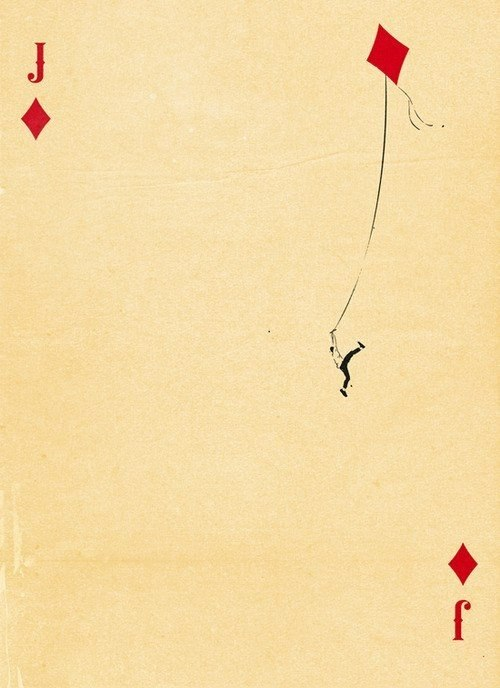
\includegraphics[width=1.28\linewidth]{Intheend}
\end{figure}
    \section*{Круглосуточный телефон идейной горячей линии:}
\begin{gather*}
 (((((20^{-i^2}\cdot (41263-6176)-1)\cdot 2-1)\cdot 2^3 -1)\cdot 2-1)\cdot 2^2 +1)\cdot 10^3 +\\+ i^2(13_{17})^{\sqrt[3]{27}} +\sqrt{16^{13}} -\Bigg(
\begin{vmatrix}{}
3 & 0 & 0 \\
37 & 14 & 7 \\
73 & 2 & 17
\end{vmatrix}
 -1 \Bigg)\cdot 10^5 +
\begin{vmatrix}{}
14 & 5 & 10 \\
0 & 0 & 1 \\
3 & 8 & 69
\end{vmatrix}
 -\\- (2-33)(17-48) + \cos^{11}\left(2\arccos\sqrt{\frac{11}{2}}\right)  -\\- 9,99329\cdot 10^{10}\cdot \left.\bigg(\frac{\partial \sin(xy)}{\partial y}\bigg)\right|_{x=1,y=0} + \\ + e^{-i\frac{\pi}{2}}\sqrt{9191 -(7\cdot 20^3+7\cdot 10^2) + 3\cdot (-5)} - \\ -
\left(\ln\left(\lim\limits_{n \rightarrow \infty}\big(1-\frac{4r^2 \arctg 1}{\sqrt{n^2}} \big)^n\right)\right)\left\{(17_{13})^{-11_2}\left[\int\limits_{-\infty}^{\infty}\exp\left(-\frac{z^2}{r^2}\right)\,dz \right]^2\right\}^{-1},
\end{gather*}

где $17_{13}$ -- это 17 в 13-тиричной системе счисления.

\begin{figure}[ht!]
    \centering
    
\includegraphics[width=\textwidth]{tony}
    \caption{Нам нужны твои идеи!}
\end{figure}

    % - может растянуть на всю страницу?
% - пока сделал только так
\begin{figure}[ht!]
    \centering
    \vspace*{-1.7cm}\hspace*{-3.2cm}
    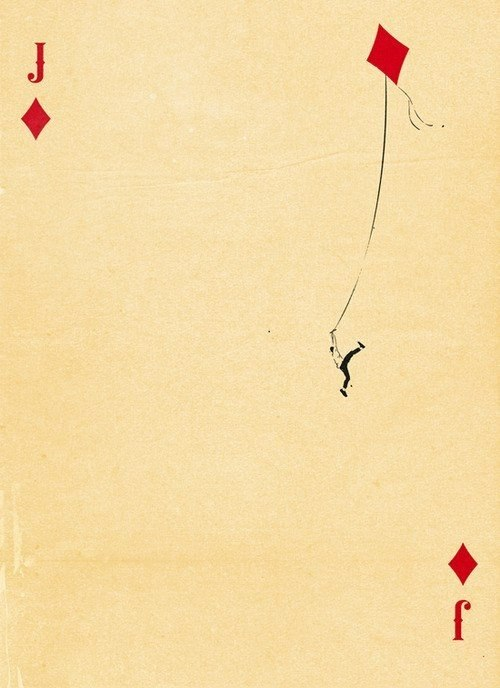
\includegraphics[width=1.28\linewidth]{Intheend}
\end{figure}

\end{document}
